\chapter{Theory of parts and wholes}\label{ch:theory-of-parts-and-wholes}

Given the conceptual background described in the previous chapter, an account for subatomic quantification is supposed to capture the intuitive notions of parthood and integrity. In this chapter, I will introduce a theory of parts and wholes that provides the formal apparatus devised to model both concepts. This theory is usually referred to as mereotopology and as suggested by the name it involves two interrelated components. In the following sections, I will first introduce standard mereology, its axioms, and advantages. Next, I will turn to its limitations and discuss how it can be extended with topological notions such as connectedness. As a result, the sophisticated mereotopological framework to be presented will allow us to model integrated wholes as opposed to other types of entities. The mereotopological distinctions to be developed will play a crucial role in the formal account for subatomic quantification in natural language that I will propose in the next chapter.

\section{Mereology}\label{sec:mereology}

\textsc{mereology} (from the Greek $\mu\epsilon\rho o\zeta$ `part') is the study of parthood, i.e., relations between part and whole as well as between parts within a whole. It was proposed by \citet{lesniewski1916podstawy} and further developed by \citet{leonard_goodman1940calculus} and \citet{goodman1951structure} as an alternative to set theory. In particular, since set theory is founded on the notion of set membership $\in$, i.e., the relation between an element and a set, it distinguishes between a singleton set and its member, i.e. $\{a\} \neq a$. For this reason, the nominalist tradition from which mereology stems has considered set theory as ontologically suspect. In order to avoid potentially problematic ontological assumptions, mereology does not postulate abstract entities such as sets. Instead, the meronomic relation of parthood is postulated as the primitive notion of the theory. Therefore, in mereology there is no need to draw the distinction between a singleton set and its member. Though historically mereology was viewed as equivalent to a rejection of set theory, since at least \citet{eberle2012nominalistic} it has been gradually recognized that employing mereological concepts is possible irrespective of one's ontological position concerning sets.

The part-whole relation can hold between portions of masses, parts of individuals, members of groups, locations, events, times, and even abstract entities, as depicted in \tabref{tab:examples-wholes-part}  \citep[see][]{simons1987parts,winston_chaffin_herrmann1987taxonomy}. It is a prominent notion in how the world appears to be structured, how human beings perceive things and talk about things. Therefore, mereology plays an important role in ontology, cognitive psychology, and natural-language semantics. Since \citeposst{quine1960word} discussion of mass nouns as scattered objects (a clearly mereological concept), considering countability in mereological terms became standard in philosophy (see especially \citealt{sharvy1980more} for a treatment of mass definite descriptions in this spirit). However, it was \citet{link1983logical} who introduced formal mereology to linguistics in his lattice-theoretic approach to pluralities.\largerpage

\begin{table}[h!]
\centering
\begin{tabular}{ll}
\lsptoprule
\textsc{whole}   & \textsc{part}     \\ \midrule
some horses  & a subset of them          \\
a quantity of water & a portion of it         \\
John, Mary, and Bill         & John          \\
some jumping events       & a subset of them        \\
a running event from A to B         & its part from A halfway towards B  \\
a temporal interval & its initial half  \\
a spatial interval          & its northern half \\ \lspbottomrule
\end{tabular}
\caption{Examples of wholes and parts \citep[p. 12]{champollion2017parts}}
\label{tab:examples-wholes-part}
\end{table}

There are different ways in which one could spell out mereological intuitions and axiomatize the parthood relation (see, e.g., \citealt{simons1987parts,casati_varzi1999parts,varzi2016mereology} for thorough surveys of the field). However, in this chapter I will discuss only a system that gives rise to algebraic structures, i.e., sets with binary operations defined on them, which is often referred to as classical extensional mereology. For brevity, however, I will simply call it standard mereology since it is considered to be a standard in mereology (though see, e.g., \citealt{rescher1955axioms} for an alternative proposal) and is most commonly used in formal semantics for natural language (e.g., \citealt{link1983logical,krifka1989nominal,landman2000events,champollion2017parts}, to name just a few prominent approaches). The axiomatization of standard mereology presented here largely  follows the extensive discussions provided by \citet{simons1987parts} and \citet{casati_varzi1999parts} as well as the encyclopedic entry on linguistic applications of mereology by \citet{champollion_krifka2016mereology}. To avoid terminological confusion I will follow \citet{grimm2012number} in distinguishing between \textsc{individuals}, i.e., a pre-theoretic notion regarding well-defined physical entities, and \textsc{m-individuals}, i.e., objects in the mereological sense.

The most common view on the axiomatization of mereology takes the concept of \textsc{part} ($\sqsubseteq$) to be the basic notion. The part-of relationship $\sqsubseteq$ is the primitive relation which is reflexive, transitive, and antisymmetric.\footnote{I use the symbol $\sqsubseteq$ following \citet{landman1989groupsi,landman1989groupsii,landman2000events}. Other authors use $\leq$ instead. The main motivation behind this notational decision is to avoid potential confusion with the `less than or equal to' relation between numbers.} The axioms given in \ref{ex:reflexivity}--\ref{ex:antisymmetry} constrain $\sqsubseteq$ to be a partial order.

\ex. Reflexivity \citep[p. 515; adapted]{champollion_krifka2016mereology}\label{ex:reflexivity}\\
{$\forall x[x\sqsubseteq x]$}\\
(Every thing is part of itself.)

\ex. Transitivity \citep[p. 516; adapted]{champollion_krifka2016mereology}\label{ex:transitivity}\\
{$\forall x\forall y\forall z[(x\sqsubseteq y \wedge y\sqsubseteq z) \rightarrow x\sqsubseteq z]$}\\
(Any part of any part of a thing is itself part of that thing.)

\ex. Antisymmetry \citep[p. 516; adapted]{champollion_krifka2016mereology}\label{ex:antisymmetry}\\
$\forall x\forall y[(x\sqsubseteq y\wedge y\sqsubseteq x)\rightarrow x=y]$\\
(Two distinct things cannot both be part of each other.)

Given that the primitive $\sqsubseteq$ relation is defined in such a way that an m-individual is part of itself, it might be useful to introduce an auxiliary notion of parthood which is not reflexive. The formula in \ref{ex:proper-part} provides the definition of \textsc{proper part} ($\sqsubset$).

\ex. Proper part \citep[p. 36]{casati_varzi1999parts}\label{ex:proper-part}\\
$x \sqsubset y \eqdef x \sqsubseteq y \wedge \neg(y \sqsubseteq x)$\\
(A proper part of a thing is a part of a thing that is distinct from it.)

Furthermore, one might also want to account for the fact that entities can share parts. For this reason, an ancillary relation \textsc{overlap} (\cnst{o}) can be defined, as in \ref{ex:overlap}.\footnote{I use the $\cnst{o}(x,y)$ notation following \citet{casati_varzi1999parts}, \citet{varzi2007spatial}, and \citet{grimm2012number}. Other authors use $x \circ y$ instead.} From a mereological point of view, identity can be understood as a special case of overlap.

\ex. Overlap \citep[p. 516; adapted]{champollion_krifka2016mereology}\label{ex:overlap}\\ 
$\cnst{o}(x,y) \eqdef \exists z[z \sqsubseteq x \wedge z \sqsubseteq y]$\\
(Two things overlap if and only if they share a part.)

The parthood relation together with the derived notions of proper part and overlap constitute the core of standard mereology. However, without any further constraints the system developed so far gives rise to structures which have been traditionally dismissed as objects that a theory of part-whole relations should represent. For instance, \figref{fig:object-solitary-proper-part} illustrates a mereological relation between the m-individuals $a$ and $b$ such that $b$ is a proper part of $a$ and there is no other proper part of $a$.\footnote{The line represents $\sqsubseteq$ with the m-individual corresponding to the lower node being part of the m-individual corresponding to the higher node.} 

\begin{figure}[h!]
\centering
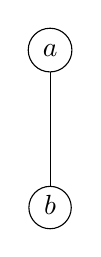
\begin{tikzpicture}[every node/.style={draw=black,thin,circle,inner sep=1pt,font=\strut}, node distance=2cm]
  \node (a) {$a$};
  \node (b) [below of=a] {$b$};
  \draw (a) -- (b);
\end{tikzpicture}
\caption{Object with a solitary proper part}
\label{fig:object-solitary-proper-part}
\end{figure}

Similarly, \figref{fig:objects-share-all-parts} depicts a model in which two distinct m-individuals $a$ and $c$ both share all parts. Though such models are allowed within the system, intuitively they are not what a theory of parts and wholes should account for. To remedy this, further constraints have to be introduced. 

\begin{figure}[h!]
\centering
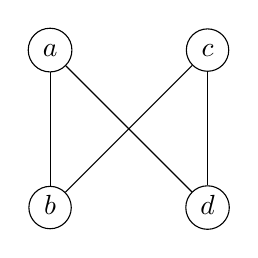
\begin{tikzpicture}[every node/.style={draw=black,thin,circle,inner sep=1pt,font=\strut}, node distance=2cm]
  \node (a) {$a$};
  \node (b) [below of=a] {$b$};
  \node (c) [right of=a] {$c$};
  \node (d) [right of=b] {$d$};
  \draw (a) -- (b);
  \draw (a) -- (d);
  \draw (b) -- (c);
  \draw (c) -- (d);
\end{tikzpicture}
\caption{Objects sharing all parts}
\label{fig:objects-share-all-parts}
\end{figure}

Standard mereology can be devised in order to restrict how an m-individual can be decomposed into parts. In particular, an additional axiom can be added that constrains mereological objects in such a way that every proper part must be supplemented by another disjoint part. In other words, there is always a mereological difference between a whole and its proper parts. An extension known as \textsc{remainder principle} or \textsc{supplementation}, see \ref{ex:supplementation}, guarantees that m-individ\-uals cannot consist of a single proper part, and thus models such as that in  \figref{fig:object-solitary-proper-part} are ruled out.\largerpage[2]

\ex. Supplementation \citep[p. 36]{casati_varzi1999parts}\label{ex:supplementation}\\
$x \sqsubset y \rightarrow \exists z[z \sqsubseteq y \wedge \neg\cnst{o}(z,x)]$\\
(Whenever a thing has a proper part, it has more than one.)

However, supplementation is insufficient to exclude structures like the one in \figref{fig:objects-share-all-parts}, and thus another extension needs to be implemented in order to ban them. Given $\sqsubseteq$, the notion of \cnst{sum} can be defined. Sums are devised to capture a pretheoretical concept of collections, i.e., the result of grouping several entities together. In natural language, conjoined terms and definite descriptions like \textit{the water} have been analyzed in terms of sums. In particular, in his influential paper \citet{link1983logical} treats expressions such as \textit{John and Mary} as referring to the sum of two individuals, namely John and Mary. In a similar vein, \citet{sharvy1980more} proposes that a definite expression such as \textit{the water} denotes the sum of all water. Here I will follow the classical definition of sum due to \citet{tarski1929fondements}, as presented in \ref{ex:sum} (for alternative definitions, see \citealt{simons1987parts,casati_varzi1999parts}).

\ex. Sum\label{ex:sum} \citep[p. 517; adapted]{champollion_krifka2016mereology}\\
$\cnst{sum}(x,P) \eqdef \forall y[P(y) \rightarrow y \sqsubseteq x] \wedge  \forall z[z \sqsubseteq x \rightarrow \exists z'[P(z') \wedge \cnst{o}(z,z')]]$

In prose, a sum of (the things in) a set $P$ is a thing that consists of everything in $P$ and whose parts each overlap with something in $P$. Since the part structures in standard mereology are closed under sum formation, for any two individuals there is also a sum of those two individuals. This is ensured by \textsc{uniqueness of sums}, which requires two things composed of the same parts to be identical, see \ref{ex:uniqueness-sums}. This principle excludes structures such as the one in \figref{fig:objects-share-all-parts}. Since $b$ and $d$ form two different sums, namely $a$ and $c$, uniqueness of sums is violated and the model is ruled out, as desired. Notice also that introducing uniqueness of sums makes the axioms of reflexivity and antisymmetry redundant since any transitive relation that satisfies uniqueness of sums is provably reflexive and antisymmetric \citep[see][]{hovda2009classical,champollion2017parts}. The axioms have been discussed for completeness though.

\ex. Uniqueness of sums \citep[p. 517; adapted]{champollion_krifka2016mereology}\label{ex:uniqueness-sums}\\
$\forall P[P \neq \varnothing \rightarrow \exists !z\ \cnst{sum}(z,P)]$\\
(Every non-empty set has a unique sum.)

Finally, the additional notions \textsc{binary sum} and \textsc{generalized sum} can be derived, as given in \ref{ex:binary-sum} and \ref{ex:generalized-sum}, respectively.\footnote{Again, I follow \citet{landman1989groupsi,landman1989groupsii,landman2000events} in the use of the symbols $\sqcup$ and $\bigsqcup$, respectively, which correspond to the symbols $\oplus$ and $\bigoplus$ one can often find in the literature.} The former operation allows us to refer explicitly to the sum of two m-individuals, whereas the latter to the sum of an arbitrary set.

\ex. Binary sum \citep[p. 518; adapted]{champollion_krifka2016mereology}\label{ex:binary-sum}\\
$x \sqcup y \eqdef \iota z\ \cnst{sum}(z,\{x,y\})$

\ex. Generalized sum \citep[p. 518; adapted]{champollion_krifka2016mereology}\label{ex:generalized-sum}\\
$\bigsqcup X \eqdef \iota z\ \cnst{sum}(z,X)$, where $X$ is any non-empty set

Consequently, the meaning of the coordinate phrase \textit{John and Mary} can be represented as $j \sqcup m$, whereas the semantics of the definite description \textit{the water} is represented as $\bigsqcup\textsc{water}$.

Alongside philosophical arguments for standard mereology, a significant advantage of this framework is that it involves a well-understood algebraic structure. In particular, as demonstrated by \citet{tarski1935grundlegung} models delivered by mereology are essentially isomorphic to Boolean algebras with their bottom element removed, or equivalently complete semi-lattices without the null element \citep[see also][]{pontow_schubert2006mathematical}.\footnote{The reason is that standard mereology does not allow for an object that is part of everything and since the empty set is a subset of every other set, it must be eliminated.} \figref{fig:semi-lattice} gives an example of a mereological structure licensed by standard mereology. Note that it is isomorphic to the powerset of the set $\{a,b,c\}$ with the bottom element removed. 

\begin{figure}[h!]
\centering
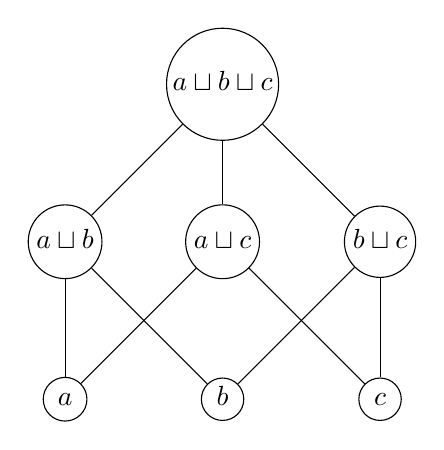
\begin{tikzpicture}[every node/.style={draw=black,thin,circle,inner sep=1pt,font=\strut}, node distance=2cm]
  \node (abc) {$a \sqcup b \sqcup c$};
  \node (ac) [below of=abc] {$a \sqcup c$};
  \node (ab) [left of=ac] {$a \sqcup b$};
  \node (bc) [right of=ac] {$b \sqcup c$};
  \node (a) [below of=ab] {$a$};
  \node (b) [right of=a] {$b$};
  \node (c) [right of=b] {$c$};
  \draw (a) -- (ab);
  \draw (a) -- (ac);
  \draw (b) -- (ab);
  \draw (b) -- (bc);
  \draw (c) -- (ac);
  \draw (c) -- (bc);
  \draw (ab) -- (abc);
  \draw (ac) -- (abc);
  \draw (bc) -- (abc);
\end{tikzpicture}
\caption{Semi-lattice}
\label{fig:semi-lattice}
\end{figure}

I will follow the well-established tradition in the semantic literature and refer to such models as complete semi-lattices. However, as pointed out by \citet{champollion2017parts} due to the lack of the null element the use of the term \textit{complete} is rather inadequate since it deviates from standard mathematical practice \citep[see also][]{landman1989groupsi}. The definition of such a structure is given in \ref{ex:complete-semi-lattice}.

\ex. Semi-lattice \citep[p. 17; adapted]{champollion2017parts}\\
Let $S$ be a set and $\sqsubseteq$ be a relation from $S$ to $S$. A pair $\langle S,\sqsubseteq \rangle$ is called a complete semi-lattice iff $\sqsubseteq$ satisfies the axioms of transitivity and uniqueness of sums.\label{ex:complete-semi-lattice}

Before we move on to the discussion of the limits of standard mereology that seem to have posed some serious problems in the study of natural language semantics adopting lattice-theoretic approaches, let us briefly contemplate some correspondences between mereology and set theory.

\subsection{Mereology vs. set theory}\label{sec:mereology-set-theory}

It can be easily noted that the notion of parthood in standard mereology has basically the same properties as the subset relation in standard set theory. Therefore, since $\sqsubseteq$ and $\subseteq$ are very much alike, there are a number of deep correspondences between the two axiom systems, some of which are illustrated in \tabref{tab:correspondences-mereology-set-theory}. Consequently, in many contexts it might be convenient to regard sums as sets, and a question arises on why mereology is preferable over set theory in modeling pluralities in natural language semantics.

\begin{table}[h]
\fittable{\begin{tabular}{lll}
\lsptoprule
\textsc{property}          & \textsc{mereology}    & \textsc{set theory}     \\ \midrule
reflexivity       & $x \sqsubseteq x$  & $x \subseteq x$ \\
transitivity      & $x \sqsubseteq y \wedge y \sqsubseteq z \rightarrow x \sqsubseteq z$     & $x \subseteq y \wedge y \subseteq z \rightarrow x \subseteq z$               \\
antisymmetry      & $x \sqsubseteq y \wedge y \sqsubseteq x \rightarrow x = y$                            & $x \subseteq y \wedge y \subseteq x \rightarrow x = y$               \\
interdefinability & $x \sqsubseteq y \Leftrightarrow x \sqcup y = y$                               & $x \subseteq y \Leftrightarrow x \cup y = y$                \\
unique sum/union  & $P \neq \varnothing \rightarrow \exists !z[\cnst{sum}(z,P)]$           & $\exists !z[z = \cup P]$               \\
associativity     & $x \sqcup (y \sqcup z) = (x \sqcup y) \sqcup z$                 & $x\cup (y\cup z)=(x\cup y)\cup z$               \\
commutativity     & $x \sqcup y = y \sqcup x$                                           & $x \cup y = y \cup x$               \\
idempotence       & $x \sqcup x = x$                                                      & $x \cup x = x$               \\
unique separation & $x \sqsubset y \rightarrow \exists !z[x\sqcup z = y \wedge \neg \cnst{o}(x,z)]$ & $x \subset y \rightarrow \exists !z[z = y - x]$ \\ \lspbottomrule
\end{tabular}}
\caption{Correspondences between mereology and set theory \citep[p. 519; adapted]{champollion_krifka2016mereology}}
\label{tab:correspondences-mereology-set-theory}
\end{table}

\begin{sloppypar}
Though early approaches to the semantics of plural expressions were grounded in set theory \citep{bennet1974some,hausser1974quantification}, a substantive body of contemporary research embraces systems based on the notion of parthood. The original motivation behind preferring mereology over set theory in the logic of plurality developed by \citet{link1983logical,link1998algebraic} was formulated on philosophical grounds. In particular, \citeauthor{link1998algebraic} argues that the traditional set-up of semantics taking the domain of individuals to be simply a non-empty set fails to represent various relations between objects. In other words, it is devised to capture only flat domains and cannot account for structured domains, as in modeling natural language. In terms of ontology, \citeauthor{link1998algebraic} describes his position as ``relative nominalism'' and argues that a set-theoretic approach is not desirable because by treating pluralities as sets, it commits us to assuming additional abstract objects. On the other hand, since in a mereological framework pluralities are treated on par with singularities as individuals, such an approach bears no additional ontological commitments, and thus is to be preferred.\footnote{But see \citet{landman1989groupsi} for a discussion challenging such a view.}
\end{sloppypar}

Another arguable advantage of using mereology rather than set theory in plural semantics is that it conveniently allows us to distinguish type-theoretically between the denotations of common nouns, i.e., set-denoting expressions of type $\langle e,t\rangle$, and plural individuals, i.e., individual-denoting expressions of type $e$ \citep[see also][]{vaillette2001flexible,champollion2017parts}. Due to the lack of sums set-theoretic approaches to pluralities conflate the meanings of these two types of expressions which can be considered an undesired result. 

A prominent linguistic application of standard mereology is the theory developed by \citet{champollion2017parts}, who adopts the order-theoretic perspective and treats $\sqsubseteq$ as primitive. On the other hand, \citet{krifka1998origins} derives $\sqsubseteq$ from $\sqcup$. Other influential theories that were intended to characterize standard mereology were developed by \citet{link1983logical,link1998algebraic} and \citet{landman1989groupsi,landman1991structures,landman2000events}.\footnote{But see a scrupulous review by \citet{hovda2009classical} who demonstrates in detail that these systems contain certain flaws, which result in them failing to describe standard mereology, as intended.}

\subsection{Limits of mereology}\label{sec:limits-of-mereology}

As has been pointed out by many authors, there is independent motivation for extending standard mereology with auxiliary notions. One factor concerns the criticism mereology faced with respect to its inadequacy in modeling objects in the real world. In particular, mereology is committed to unrestricted sum formation and as such it is insufficient to capture what it means to be a whole. This results in diametrical discrepancies between intuitions regarding the nature of entities in the world and objects mereology actually delivers. To use \citeposst{casati_varzi1999parts} example, imagine a cup and broken glass. Intuitively, the former constitutes an object, i.e., an individuated whole, something that counts as one, whereas the latter is just a collection of shards. However, this distinction cannot be captured by describing entities purely in terms of parthood. This is because in mereology for every whole there is a set of parts and to every arbitrary collection of parts there is their sum, i.e., a complete whole. As a result, a cup and broken glass have the very same mereological status. In other words, the allowance of scattered entities makes it impossible to differentiate between them and individuals constituting integrated wholes. Consequently, mereology has faced criticism that in principle it fails as a theory of individuals.

As suggested by \citet{grimm2012number}, it is very likely that at least some of the shortcomings of mereological approaches to pluralities and countability in natural language may be due to the general flaws of standard mereology in attempting to capture what it means to be a whole. Arguably, extending standard mereological frameworks with additional notions in order to develop a better theory of objects, as proposed, e.g., by \citet{casati_varzi1999parts}, may provide superior tools for semantic treatments of quantification in natural language. As already signaled, a challenging problem concerns the requirement of unrestricted sum formation which states that for every two elements in the domain, there is a plural individual corresponding to the sum of those two elements. Specifically, the ontological status of such a plural entity has often been disputed. As wittily put by \citet{landman1989groupsi}, if three children messed up the living room, the correct answer to the question ``How many individuals were involved in messing up the living room?'' is ``three'', whereas ``seven'' clearly seems incorrect.\footnote{See also \citet{cresswell1985review}.} However, if pluralities were conceptualized as having the same ontological status as singular individuals, we would expect this answer to be adequate since that number includes all distinct sums of the children in question. In other words, if the children were Anne, Betty, and Carl, i.e., $a$, $b$, and $c$ respectively, then 7 is the number of the elements of the set consisting of all entities that are part of the total sum of the children, i.e., $\{a, b, c, a \sqcup b, a \sqcup c, b \sqcup c, a \sqcup b \sqcup c\}$. The fact that natural language does not allow for quantification over arbitrary sums suggests that the way individual objects are conceptualized differs from how we see pluralities of objects. However, standard mereology lacks notions fine-grained enough to distinguish between objects that come in one piece and entities that do not.

The next section will introduce an extension of standard mereology within which more fine-grained notions can be defined. These notions will enhance mereology in that in addition to parthood they will allow us to capture also the topological configuration of entities making up a particular sum, i.e., their spatial arrangement. In other words, the topological extension will make it possible to discriminate between scattered entities and wholes that come in one piece.

\section{Mereotopology}\label{sec:mereotopology}

\textsc{topology} (from the Greek $\tau o\pi o\zeta$ `place') is the study of those properties of space that are unaffected by continuous deformations of shape or size of figures such as stretching or bending, as opposed to tearing or gluing. Two of the crucial notions studied in the field are connectedness and compactness. Important contributions to the early development of topology were made by \citet{frechet1906quelques}, \citet{hausdorff1914grundzuge}, and \citet{kuratowski1922operation}. 

Theories that extend standard mereology with topological relations are  known as \textsc{mereotopology}. Though early attempts to formalize such a system trace back to \citet{whitehead1920concept,whitehead1929process}, for many decades there was no continuation in the systematic study of mereotopological issues until relatively recent work in artificial intelligence began to investigate the interaction between mereological and topological notions in order to develop formal representations of spatial relations such as \textsc{near} or \textsc{inside}. Consequently, new developments in philosophy and ontological modeling  \citep[e.g.,][]{clarke1981calculus,smith1996mereotopology,roeper1997region} motivated the extension of standard mereology with topological relations in order to advance an improved theory of objects.

Though topological notions have been widely used within the study of locatives \citep[e.g.,][]{clark1973space,herskovits1985semantics,zwarts_winter1997semantic,kracht2002semantics}, it was not until \citet{grimm2012degrees,grimm2012number} that mereotopology was introduced to natural language semantics.\footnote{Mereotopology has been further applied to particular topics concerning countability in \citet{lima2014all} and \citet{grimm_docekal-toappear-counting}. The theory has also inspired approaches that do not develop full-fledged mereotopological accounts but employ some spatial relations in order to capture certain issues relating to individuation such as \citet{scontras2014semantics,scontras2017new}, \citet{sutton_filip2017probabilistic,sutton_filip2017individuation}, \citet{henderson2017swarms}, and \citet{krifka-toappear-individuating}.} In this chapter, I will define basic topological concepts and review how they interact with mereological notions as discussed by \citet{casati_varzi1999parts} and adopted for the semantic treatment of countability by \citet{grimm2012degrees,grimm2012number}.

There are two main approaches with respect to relating mereology and topology: (i)~choosing mereology as a basic level and augmenting it with topological notions, or (ii)~choosing topology as a basic level and adding mereological relations. I will follow \citet{grimm2012number}, who employs a technique of simply extending mereology with topological notions. In particular, he adopts the approach developed in \citet{casati_varzi1999parts}, which I will describe in the following paragraphs.\largerpage

The crucial topological notion for the purpose of this study is \textsc{connectedness} (\cnst{c}). This relation is introduced in such a way that it interacts with other definitions and axioms of standard mereology. Connectedness is reflexive and symmetric, as defined in the axioms in \ref{ex:connectivity-reflexivity} and \ref{ex:connectivity-symmetry}.

\ex. Reflexivity \citep[p. 52; adapted]{casati_varzi1999parts}\label{ex:connectivity-reflexivity}\\
$\forall x[\cnst{c}(x,x)]$\\
(Every thing is connected to itself.)
	
\ex. Symmetry \citep[p. 52; adapted]{casati_varzi1999parts}\label{ex:connectivity-symmetry}\\
$\forall x\forall y[\cnst{c}(x,y) \rightarrow \cnst{c}(y,x)]$\\
(If $x$ is connected to $y$, then $y$ is also connected to $x$.)

Notice, however, that unlike the parthood relation $\sqsubseteq$, as defined in standard mereology, recall \ref{ex:reflexivity}--\ref{ex:antisymmetry}, the connectedness relation \cnst{c} does not need to be transitive. For instance, consider the configuration depicted in \figref{fig:connectedness-transitivity}. Although $a$ and $b$ are connected to each other and $b$ and $c$ are connected to each other, it is not the case that $a$ and $c$ are connected to each other.

\begin{figure}[h!]
\centering
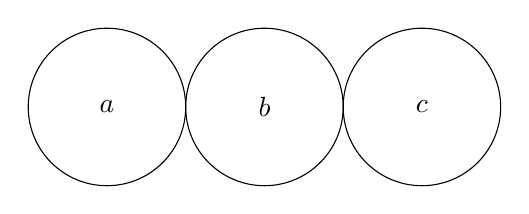
\begin{tikzpicture}
  \draw (0.0,0.0) circle (1cm);
  \draw (2.0,0.0) circle (1cm);
  \draw (4.0,0.0) circle (1cm);
  \node at (0.0,0.0) {$a$};
  \node at (2.0,0.0) {$b$};
  \node at (4.0,0.0) {$c$};
\end{tikzpicture}
\caption{Connectedness and transitivity}
\label{fig:connectedness-transitivity}
\end{figure} 

As discussed by \citet{casati_varzi1999parts}, there are a number of intuitive interactions between the topological notion $\cnst{c}$ and the mereological relations $\sqsubseteq$ and $\cnst{o}$. These intuitive interactions can be formalized as the so-called bridging principles which interrelate the mereological and the topological component of the theory (\citealt{varzi2007spatial}). The main aim of the bridging principles is to secure that, irrespective of their full characterization, $\sqsubseteq$ and $\cnst{c}$ are related in such a manner that a whole and its parts are firmly connected. In particular, the principle of \textsc{integrity} ensures that connectedness is implied by parthood, see \ref{ex:integrity}, and consequently mereological overlap is in fact a form of connection, as guaranteed by the principle of \textsc{unity}, see \ref{ex:unity}. Finally, the principle defined in \ref{ex:monotonicity} secures \textsc{monotonicity}.\footnote{In fact, \ref{ex:monotonicity} implies both \ref{ex:integrity} and \ref{ex:unity} \citep[pp. 981--982]{varzi2007spatial}. However, I provide all the bridging principles for the sake of completeness.}

	\ex. Integrity \citep[p. 981; adapted]{varzi2007spatial}\label{ex:integrity}\\
    $\forall x\forall y[x \sqsubseteq y \rightarrow \cnst{c}(x,y)]$\\
(If an m-individual is part of another m-individual, then they are connected.)

\ex. Unity \citep[p. 981; adapted]{varzi2007spatial}\label{ex:unity}\\
$\forall x\forall y[\cnst{o}(x,y) \rightarrow \cnst{c}(x,y)]$\\
(If two m-individuals overlap, then they are connected.)

\ex. Monotonicity \citep[p. 981; adapted]{varzi2007spatial}\label{ex:monotonicity}\\
$\forall x\forall y\big[x \sqsubseteq y \rightarrow \forall z [\cnst{c}(z,x) \rightarrow \cnst{c}(z,y)]\big]$\\
(If an m-individual is part of another m-individual, then whatever is connected to the former, is also connected to the latter.)

Given these extensions, a number of mereotopological properties like \textsc{internal part} (\cnst{ip}), \textsc{internal overlap} (\cnst{io}), and \textsc{tangential overlap} (\cnst{to}) can be defined. Such notions enable us to draw subtle topological distinctions in order to account for different spatial configurations that entities may be in. For instance, the individual $b$ in \figref{fig:internal-part} is an internal part of the individual $a$ since every entity that is connected to $b$ overlaps with $a$ or, in other words, $a$ includes $b$. On the other hand, though part of $b$ is an internal part of $a$ in \figref{fig:internal-overlap}, there is also a part of $b$ which is not included in $a$. Finally, \figref{fig:tangential-overlap} illustrates a configuration where there is overlap between $a$ and $b$ but there is no internal overlap, i.e., the individuals only share their edges.

\begin{figure}[h!]
\begin{floatrow}
\captionsetup{margin=.05\linewidth}
\ffigbox[.33\textwidth]{\caption{Internal part}\label{fig:internal-part}}
        {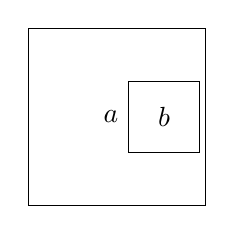
\begin{tikzpicture}[scale=.75]
           \node at (1.4,1.5) {$a$};
           \node at (2.3,1.5) {$b$};
           \draw (0,0) -- (0,3) -- (3,3) -- (3,0) -- (0,0);
           \draw (1.7,2.1) -- (2.9,2.1) -- (2.9,0.9) -- (1.7,0.9) -- (1.7,2.1);
         \end{tikzpicture}}
\ffigbox[.33\textwidth]{\caption{Internal overlap}\label{fig:internal-overlap}}
         {\begin{tikzpicture}[scale=.75]
           \node at (1.5,1.5) {$a$};
           \node at (3.3,1.5) {$b$};
           \draw (0,0) -- (0,3) -- (3,3) -- (3,0) -- (0,0);
           \draw (2.7,2.1) -- (3.9,2.1) -- (3.9,0.9) -- (2.7,0.9) -- (2.7,2.1);
         \end{tikzpicture}}
\ffigbox[.33\textwidth]{\caption{Tangential overlap}\label{fig:tangential-overlap}}
        {\begin{tikzpicture}[scale=.75]
         \node at (1.5,1.5) {$a$};
         \node at (3.6,1.5) {$b$};
         \draw (0,0) -- (0,3) -- (3,3) -- (3,0) -- (0,0);
         \draw (3,2.1) -- (4.2,2.1) -- (4.2,0.9) -- (3,0.9) -- (3,2.1);
         \end{tikzpicture}}
\end{floatrow}
\end{figure}

The relevant definitions are given in \ref{ex:internal-part}--\ref{ex:tangential-overlap}.

\ex. Internal part \citep[p. 55; adapted]{casati_varzi1999parts}\label{ex:internal-part}\\
$\cnst{ip}(x,y) \eqdef x \sqsubseteq y \wedge \forall z[\cnst{c}(z,x) \rightarrow \cnst{o}(z,y)]$

\ex. Internal overlap \citep[p. 55; adapted]{casati_varzi1999parts}\label{ex:internal-overlap}\\
$\cnst{io}(x,y) \eqdef \exists z[\cnst{ip}(z,x) \wedge \cnst{ip}(z,y)]$

\ex. Tangential overlap \citep[p. 55; adapted]{casati_varzi1999parts}\label{ex:tangential-overlap}\\
$\cnst{to}(x,y) \eqdef \cnst{o}(x,y) \wedge \neg \cnst{io}(x,y)$

In addition, within the mereotopological framework standard topological notions can be defined. Assuming \textsc{mereological complement} (${\sim}$), as provided in \ref{ex:mereological-complement}, \ref{ex:interior}--\ref{ex:boundary} give definitions for \textsc{interior} (\cnst{int}), \textsc{exterior} (\cnst{ext}), \textsc{closure} (\cnst{clo}), and \textsc{boundary} (\cnst{b}), respectively.   

\ex. Mereological complement\label{ex:mereological-complement} \citep[p. 45; adapted]{casati_varzi1999parts}\\
${\sim}(x) \eqdef \iota y\forall z[z \sqsubseteq y \leftrightarrow \neg\cnst{o}(z,x)]$

\ex. Interior\label{ex:interior} \citep[p. 58; adapted]{casati_varzi1999parts}\\
$\cnst{int}(x) \eqdef \sqcup X$ where $X = \{y\ :\ \cnst{ip}(y,x) = \cnst{true}\}$

\ex. Exterior\label{ex:exterior} \citep[p. 58; adapted]{casati_varzi1999parts}\\
$\cnst{ext}(x) \eqdef \cnst{int}({ \sim} (x))$

\ex. Closure\label{ex:closure} \citep[p. 58; adapted]{casati_varzi1999parts}\\
$\cnst{clo}(x) \eqdef { \sim}(\cnst{ext}(x))$

\ex. Boundary\label{ex:boundary} \citep[p. 58; adapted]{casati_varzi1999parts}\\
$\cnst{b}(x) \eqdef { \sim}(\cnst{int}(x) \sqcup \cnst{ext}(x))$

\figref{fig:interior}--\ref{fig:closure} illustrate the intended configurations.

\begin{figure}
\begin{floatrow}
  \captionsetup{margin=.05\linewidth}
  \ffigbox[.33\textwidth]{\begin{tikzpicture}
  \draw (0,0) -- (0,3) -- (3,3) -- (3,0) -- (0,0);
  \draw[dashed,pattern=south east lines,pattern color=gray!25] (1.5,1.5) circle (1cm);
  \node at (1.5,1.5) {$a$};
  \end{tikzpicture}}
  {\caption{Interior\label{fig:interior}}}
  \ffigbox[.33\textwidth]{\begin{tikzpicture}
  \draw[pattern=south east lines,pattern color=gray!25] (0,0) -- (0,3) -- (3,3) -- (3,0) -- (0,0);
  \draw[dashed,fill=white] (1.5,1.5) circle (1cm);
  \node at (1.5,1.5) {$a$};
   \end{tikzpicture}}
   {\caption{Exterior\label{fig:exterior}}}
  \ffigbox[.33\textwidth]{\begin{tikzpicture}
  \draw (0,0) -- (0,3) -- (3,3) -- (3,0) -- (0,0);
  \draw[pattern=south east lines,pattern color=gray!25] (1.5,1.5) circle (1cm);
  \node at (1.5,1.5) {$a$};
  \end{tikzpicture}}
  {\caption{Closure\label{fig:closure}}}
\end{floatrow}
\end{figure}

\iffalse

\begin{figure}[h!]
\RawFloats
\centering
\begin{minipage}[b]{.49\textwidth}
\centering
\begin{tikzpicture}
  \draw (0,0) -- (0,3) -- (3,3) -- (3,0) -- (0,0);
  \draw[dashed,pattern=south east lines,pattern color=gray!25] (1.5,1.5) circle (1cm);
  \node at (1.5,1.5) {$a$};
\end{tikzpicture}
\caption{Interior}
\label{fig:interior}
\end{minipage}
\begin{minipage}[b]{.49\textwidth}
\centering
\begin{tikzpicture}
  \draw[pattern=south east lines,pattern color=gray!25] (0,0) -- (0,3) -- (3,3) -- (3,0) -- (0,0);
  \draw[dashed,fill=white] (1.5,1.5) circle (1cm);
  \node at (1.5,1.5) {$a$};
\end{tikzpicture}
\caption{Exterior}
\label{fig:exterior}
\end{minipage}
~
\begin{minipage}[b]{1.0\textwidth}
\vspace{1.0ex}
\centering
\begin{tikzpicture}
  \draw (0,0) -- (0,3) -- (3,3) -- (3,0) -- (0,0);
  \draw[pattern=south east lines,pattern color=gray!25] (1.5,1.5) circle (1cm);
  \node at (1.5,1.5) {$a$};
\end{tikzpicture}
\caption{Closure}
\label{fig:closure}
\end{minipage}
\end{figure}

\fi

The shaded area in \figref{fig:interior} represents the interior of an object, which is taken to be the sum of an m-individual's internal parts. The dashed line marks the boundary of the object, i.e., the part that is not included in its interior. On the other hand, \figref{fig:exterior} represents the exterior of an object, which again does not comprise the boundary, whereas the solid line in \figref{fig:closure} indicates that both the interior and boundary make up the closure of an entity.

The framework described so far extends standard mereology with the primitive topological relation of connectedness and several derived notions, which allow us to talk about different configurations that entities can be in. Such a system provides means to distinguish between arbitrary and non-arbitrary sums, and consequently to define individuals as integrated wholes, i.e., objects characterized in terms of different degrees of connectedness. The following section will discuss a mereotopological approach to such individuals.

\subsection{Integrated wholes}\label{sec:integrated-wholes}

A great advantage of the mereotopological approach to natural language semantics is that by means of the topological relations defined so far it is possible to capture what it means to be an individual understood as an integrated whole. In particular, a distinction can be drawn between entities which come in one piece, as opposed to pluralities, i.e., scattered entities, which bear no topological commitments. To distinguish the former from the latter, it is essential to introduce the property \textsc{self-connected} (\cnst{sc}). Unlike arbitrary sums, \cnst{sc} entities cannot be divided into separated parts. The definition of \cnst{sc} is provided in \ref{ex:self-connected}.
	
	\ex. Self-connected \citep[p. 57; adapted]{casati_varzi1999parts}\label{ex:self-connected}\\
    $\cnst{sc}(x) \eqdef \forall y \forall z[\forall w(\cnst{o}(w,x) \leftrightarrow (\cnst{o}(w,y) \vee \cnst{o}(w,z))) \rightarrow \cnst{c}(y,z)]$\\
	(An entity is self-connected if and only if any two parts that form the whole of that entity are connected to each other.)
	
    Given the definition in \ref{ex:self-connected}, it is possible to differentiate inseparable individuals from separable ones including arbitrary sums of entities, i.e., disconnected configurations of objects. To illustrate this let us assume a model containing four entities. Specifically, suppose $a$ and $b$ are two halves of a cube, whereas $c$ and $d$ are a pyramid and a sphere, respectively, see \figref{fig:wholes-sums}. Intuitively, there is a difference between the sum $s_1 = a \sqcup b$ and the sum $s_2 = c \sqcup d$. While $s_1$ forms an integrated whole, the plurality $s_2$ is just an arbitrary collection of disconnected objects, and thus it does not make up a solid whole. In other words, $\cnst{sc}(s_1)$ is true, whereas $\cnst{sc}(s_2)$ is false. 
    
\begin{figure}[h!]
\centering
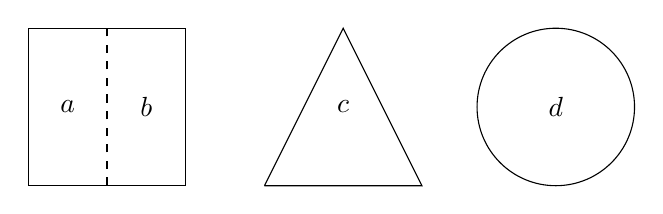
\begin{tikzpicture}
  \draw (0,0) -- (2,0) -- (2,2) -- (0,2) -- (0,0);
  \draw[dashed] (1,0) -- (1,2);
  \draw (3,0) -- (4,2) -- (5,0) -- (3,0);
  \draw (6.7,1) circle (1cm);
  \node at (0.5,1) {$a$};
  \node at (1.5,1) {$b$};
  \node at (4,1) {$c$};
  \node at (6.7,1) {$d$};  
\end{tikzpicture}
\caption{Wholes vs. sums}
\label{fig:wholes-sums}
\end{figure}      
    
    Self-connectedness is a great improvement in the theory of wholeness. However, this notion is still insufficient to capture what it means to be conceptualized as an integrated object since it allows for configurations involving only an external connection holding between individuals. In other words, cases when the closure of one object overlaps the other or vice versa are not ruled out. For instance, \figref{fig:external-connection} depicts two spheres $a$ and $b$ which only touch each other, i.e., their boundaries are connected at a single point. Given the definition of \cnst{sc} in \ref{ex:self-connected}, $a$ and $b$ are self-connected but intuitively such a spatial configuration is not sufficient to count as an integrated whole.
    
\begin{figure}[h!]
\centering
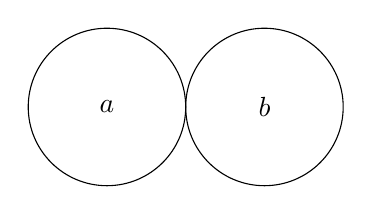
\begin{tikzpicture}
  \draw (0.0,0.0) circle (1cm);
  \draw (2.0,0.0) circle (1cm);
  \node at (0.0,0.0) {$a$};
  \node at (2.0,0.0) {$b$};
\end{tikzpicture}
\caption{External connection}
\label{fig:external-connection}
\end{figure}    
  
In order to rule out cases such as the one illustrated in \figref{fig:external-connection}, a stronger relation is required. Ostensibly, what is necessary is that not only boundaries of parts of a whole are connected to each other, but also that their internal parts are shared. To solve this problem one needs to define an additional restriction on the concept of interior given in \ref{ex:interior}. Accordingly, \citet{casati_varzi1999parts} postulate the property of being \textsc{strongly self-connected} (\cnst{ssc}), as defined in \ref{ex:strongly-self-connected}.\footnote{Notice that on some plausible assumptions concerning boundaries the first conjunct in \ref{ex:strongly-self-connected} is superfluous (for a discussion of various views on boundaries, see \citealt[pp. 61--62, 71--98]{casati_varzi1999parts}).} This refinement will get us much closer to the type of entities we would like to single out, i.e., integrated wholes.

	\ex. Strongly self-connected \citep[p. 60; adapted]{casati_varzi1999parts}\label{ex:strongly-self-connected}\\
    $\cnst{ssc}(x) \eqdef \cnst{sc}(x) \wedge \cnst{sc}(\cnst{int}(x))$\\
    (An m-individual is strongly self-connected if it is self-connected and its interior is self-connected.)
	
	The restriction introduced in \ref{ex:strongly-self-connected} guarantees that not only boundaries of parts are shared but also that the interior of an entity is self-connected. Therefore, the property of \cnst{ssc} rules out objects that merely touch each other, e.g., the spheres in \figref{fig:external-connection}. However, the fact that an entity is strongly self-connected still does not ensure that such an entity is an integrated whole in the sense a theory of wholeness is supposed to capture. For instance, consider the entity $a$, i.e., the left half of the cuboid represented in \figref{fig:strongly-self-connected-part}. Although $a$ qualifies as a strongly self-connected object since any two parts that form its interior are connected, intuitively it cannot be characterized as a whole. Obviously, the reason is that there is yet another half of the cuboid and only the two together make up the entire individual. Consequently, \cnst{ssc} is insufficient for our purposes and an even stronger notion is required to capture what is perceived as an integral whole.

\begin{figure}[h!]
\centering
\begin{tikzpicture}
  \draw (0,0) -- (2,0) -- (2,2) -- (0,2) -- (0,0);
  \draw[dashed] (1,0) -- (1,2);
  \node at (0.5,1) {$a$};
\end{tikzpicture}
\caption{Strongly self-connected part}
\label{fig:strongly-self-connected-part}
\end{figure}

	Describing wholes is about capturing an intuitive notion of unity. This means that a proper definition should accommodate both topological integrity and mereological exhaustivity. For this purpose, \citet{casati_varzi1999parts} introduce the property of being \textsc{maximally strongly self-connected} (\cnst{mssc}), as defined in \ref{ex:maximally-strongly-self-connected}.
	
	\ex. Maximally-strongly-self-connected \citep[p. 60; adapted]{casati_varzi1999parts}\label{ex:maximally-strongly-self-connected}\\
	$\cnst{mssc}(x) \eqdef \cnst{ssc}(x) \wedge \forall y[\cnst{ssc}(y) \wedge \cnst{o}(y,x) \rightarrow y \sqsubseteq x]$\\
    (An m-individual is maximally strongly self-connected if (i)~every part of the individual is connected to (overlaps) the whole (strongly self-connect\-ed) and (ii)~anything else which overlaps it and is strongly self-connected is once again part of it (maximality).)

	More generally one could single out entities that are maximally strongly self-connected relative to a particular property. The relativized \cnst{mssc} property can be characterized as in \ref{ex:maximally-strongly-self-connected-relative}, which provides the final mereotopological definition of what an integrated whole is.
	
	\ex. Maximally strongly self-connected relative to a property \citep[p. 60; adapted]{casati_varzi1999parts}\label{ex:maximally-strongly-self-connected-relative}\\
	$\cnst{mssc}(P)(x) \eqdef P(x) \wedge \cnst{ssc}(x) \wedge \forall y[P(y) \wedge \cnst{ssc}(y) \wedge \cnst{o}(y,x) \rightarrow y \sqsubseteq x]$\\
     (An m-individual is maximally strongly self-connected relative to a property if (i) every part of the individual is connected to (overlaps) the whole (strongly self-connected) and (ii) anything else which has the same property, is strongly self-connected, and overlaps it is once again part of it (maximality).)
	
	If an entity satisfies \cnst{mssc}, then it is the largest entity satisfying that property which is self-connected. For instance, if $P$ is the property of being a cuboid, then the definition in \ref{ex:maximally-strongly-self-connected-relative} will select the largest such entities among those that come in one piece. In particular, it will single out the whole cuboid in \figref{fig:strongly-self-connected-part} as opposed to, e.g., its left half $a$ though $a$ itself also satisfies the property of being a cuboid. That is because $a$ is part of the cuboid whereas the whole cuboid is not part of any other strongly self-connected object.
    
    Though the structure of the mereotopological framework of \citet{casati_varzi1999parts} discussed above is relatively simple, the distinctions developed within it are fine-grained enough for the representation of spatial objects. As standard mereology, mereotopology gives rise to algebraic structures isomorphic to \linebreak Boolean algebras with their bottom element removed. However, such lattice representations are further endowed with regions indicating which elements are associated with the connectedness relation \cnst{c}. For instance, consider \figref{fig:parthood-and-connectedness}. 
     
    \begin{figure}[h!]
\centering
\begin{tikzpicture}[node distance=2cm]
  \node[draw=black,thin,circle,inner sep=3pt] (abc) {$a \sqcup b \sqcup c$};
  \node[draw=black,thin,circle,inner sep=3pt] (ac) [below of=abc] {$a \sqcup c$};
  \node[draw=black,thin,circle,inner sep=3pt] (ab) [left of=ac] {$a \sqcup b$};
  \node[draw=black,thin,circle,inner sep=3pt] (bc) [right of=ac] {$b \sqcup c$};
  \node[draw=black,thin,circle,inner sep=3pt] (a) [below of=ab] {$a$};
  \node[draw=black,thin,circle,inner sep=3pt] (b) [right of=a] {$b$};
  \node[draw=black,thin,circle,inner sep=3pt] (c) [right of=b] {$c$};
  \draw (a) -- (ab);
  \draw (a) -- (ac);
  \draw (b) -- (ab);
  \draw (b) -- (bc);
  \draw (c) -- (ac);
  \draw (c) -- (bc);
  \draw (ab) -- (abc);
  \draw (ac) -- (abc);
  \draw (bc) -- (abc);
  \draw[thick,dashed,pattern=south east lines,pattern color=gray!25] (-2.8,-1.25) -- (-2.8,-4.6) -- (0.6,-4.6) -- (0.6,-3.65) -- (-1.65,-1.25) -- (-2.8,-1.25); 
  \draw[<->] (-3.2,0.9) -- (-3.2,-4.6);
  \draw[<->] (-2.8,-5.0) -- (2.8,-5.0);
  \node at (0.0,-5.4) {connectedness};
  \node[rotate=90] at (-3.6,-2.1) {parthood};
\end{tikzpicture}
\caption{Parthood and connectedness \citep[based on][p. 136]{grimm2012number}}
\label{fig:parthood-and-connectedness}
\end{figure}

Given a model with 3 entities, namely two halves of a cube $a$ and $b$ and a pyramid $c$, the semi-lattice represents all the possible sums generated by the set of corresponding m-individuals. The vertical axis illustrates the parthood relation with individual lines between particular nodes symbolizing $\sqsubseteq$, whereas the horizontal axis represents connectedness. The shaded area then covers those entities in the structure which are connected. In other words, the mereological component of the theory defines part-whole relations between $a$, $b$, and $c$ and all the possible sums thereof, whereas the topological component singles out those parts that form self-connected wholes. In particular, while $a$ in the model is part of $a \sqcup b$ (as well as of itself due to the axiom of reflexivity), it is not part of $b$. However, it is connected to $b$ (as well as to $a \sqcup b$ due the axiom of integrity and to itself -- again reflexivity).
   
    Moreover, as discussed by \citet{grimm2012number}, the subtle niceties between different types of connectedness provide means to capture differences between distinct types of nominals, such as object, substance, and aggregate nouns, as well as eliminate old problems concerning cumulative singular count nouns such as \textit{fence} or \textit{twig} \citep[see, e.g.,][]{zucchi_white2001twigs,rothstein2010counting}. Specifically, among multiple parts that have a property of being, say, a rock only the maximal (improper) part counts as a whole object. Hence, I conclude that compared to standard mereology, mereotopology proves to be a superior theory of parts and wholes and its application in natural language semantics should be considered advantageous. In the next section I will discuss several other kinds of connection. 

\subsection{Other types of connection}\label{sec:other-types-of-connection}

In the previous section, we saw that given the primitive relation \cnst{c} it is possible to derive a notion that can capture what it means to be an integrated whole as opposed to an arbitrary sum, namely the \cnst{mssc} property. This, however, does not deplete the potential of mereotopology in modeling different types of objects and spatial configurations. Based on \cnst{c}, many other types of topological relations representing distinct varieties of connectedness may be defined. In this section, I will discuss some of them.

\begin{sloppypar}
The first auxiliary mode of connection to be discussed is the property of \textsc{firmly connected} (\cnst{fc}), as defined in \ref{ex:firmly-connected}.\footnote{I use the term following \citet{varzi2007spatial}, whereas \citet{casati_varzi1999parts} and \citet{grimm2012degrees,grimm2012number} talk about strong connection. My motivation is mainly to avoid potential confusion with the \cnst{ssc} property which plays a crucial role in defining \cnst{fc} but is distinct from it.} 
\end{sloppypar}

\ex. Firmly connected \citep[p. 1003; adapted]{varzi2007spatial}\label{ex:firmly-connected}\\
$\cnst{fc}(x,y) \eqdef \exists w \exists z[w \sqsubseteq x \wedge z \sqsubseteq y \wedge \cnst{ssc}(w \sqcup z)]$\\
(Two m-individuals are firmly connected if a sum of their parts is strongly self-connected.)

This property holds between two entities when they overlap in a substantive sense. In other words, two m-individuals are firmly connected if their sum is strongly self-connected. Such a definition excludes cases of tangential overlap, i.e., configurations where entities only touch each other, since the \cnst{ssc} property implies that not only the boundaries but also the interiors of m-individuals are connected.

With an additional restriction regarding the local scope of connectedness, the notion of \cnst{fc} seems to be suitable to capture what it means to be conceptualized as a substance, as opposed to an integrated individual that we count as one. Specifically, substances can be represented as comprising of m-individuals that are locally firmly connected, i.e., at a given location an instance of a substance is always firmly connected to another instance of the same substance \citep[pp. 140--142]{grimm2012degrees,grimm2012number}. For instance, a section of mud in a puddle overlaps with other sections of the puddle of mud, which are again mud.  

In contrast to \cnst{fc}, the property \textsc{externally connected} (\cnst{ec}), as defined in \ref{ex:externally-connected}, concerns entities that are merely tangentially connected, i.e., it is only their boundaries that are connected, whereas their interiors do not overlap. This notion enables us to model configurations of entities that are not merged but simply touch each other.

\ex. Externally connected \citep[p. 134; adapted]{grimm2012number}\label{ex:externally-connected}\\
$\cnst{ec}(x,y) \eqdef \cnst{c}(x,y) \wedge \neg \cnst{c}(\cnst{int}(x),\cnst{int}(y))$\\
(Two m-individuals are externally connected if they are connected but it is not the case that their interiors are connected.)

Another topological notion it might be useful to derive is one describing a configuration of objects touching each other in such a way that they form, say, a row. This variety of connectedness can be captured by the property \textsc{by-connected} (\cnst{bc}), as provided by \citet{varzi2007spatial}. It holds between entities that are not connected to each other but are associated by virtue of being connected to another mediating entity. The definition in \ref{ex:by-connected} describes \cnst{bc} as a three-place relation establishing indirect connectedness between the outermost entities within a configuration.

\ex. By-connected \citep[p. 979; adapted]{varzi2007spatial}\label{ex:by-connected}\\
$\cnst{bc}(x,y,z) \eqdef \cnst{c}(x,z) \wedge \cnst{c}(z,y)$\\
(Three m-individuals $x$, $y$, and $z$ are by-connected if $x$ is connected to $z$ and $z$ is connected to $y$.)

A related notion is called \textsc{mediately connected} (\cnst{mc}). This is a binary relation that holds between entities that are not necessarily connected to each other, but are part of a by-connected configuration, e.g, a row of individuals. In other words, there is an object that mediates the connection between two such entities. The formal definition of \cnst{mc} is given in \ref{ex:mediately-connected}.

\ex. Mediately connected \citep[p. 979; adapted]{varzi2007spatial}\label{ex:mediately-connected}\\
$\cnst{mc}(x,y) \eqdef \exists z [\cnst{bc}(x,y,z)]$\\
(Two m-individuals are mediately connected if they are by-connected through a third m-individual.)

\pagebreak To illustrate the \cnst{bc} and \cnst{mc} relations, consider the configuration of two spheres $a$ and $c$ and a cube $b$, as depicted in  \figref{fig:by-connected-and-mediately-connected}. The three entities are by-connected since $a$ is externally connected to $b$ and $b$ is externally connected to $c$. At the same time, the spheres are mediately connected since both $a$ and $c$ are connected to the cube $b$, i.e., $b$ in a way mediates the connection between $a$ and $c$.

\begin{figure}[h!]
\centering
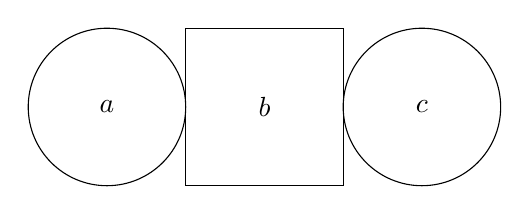
\begin{tikzpicture}
  \draw (0.0,0.0) circle (1cm);
  \draw (1.0,-1.0) -- (3.0,-1.0) -- (3.0,1.0) -- (1.0,1.0) -- (1.0,-1.0);
 \draw (4.0,0.0) circle (1cm);
  \node at (0.0,0.0) {$a$};
  \node at (2.0,0.0) {$b$};
  \node at (4.0,0.0) {$c$};
\end{tikzpicture}
\caption{By-connected and mediately connected}
\label{fig:by-connected-and-mediately-connected}
\end{figure}

As pointed out by \citet[pp. 134--135]{grimm2012number}, the notion of \cnst{mc} may prove useful in modeling natural language expressions denoting entities such as eyes or fingers. Such objects seem to be conceptualized in a particular way which is further reflected in grammar. Specifically, in some languages they belong to a category of inherently plural or dual expressions.

Furthermore, the \cnst{bc} relation can be generalized to hold for any number of entities. This gives rise to the property \textsc{transitively connected} (\cnst{tc}). As defined in \ref{ex:transitively-connected} \citep[see][p. 144]{grimm2012degrees,grimm2012number}, it is intended to determine whether two individuals are connected through a series of mediating entities. For instance, it would hold of two opposite entities in a scenario similar to the one illustrated in  \figref{fig:by-connected-and-mediately-connected} with the exception that between the spheres $a$ and $c$ there is not only the cube $b$, but also a pyramid $d$ such that it touches both $b$ an $c$.

\ex. Transitively connected \citep[p. 15; adapted]{grimm2012degrees}\label{ex:transitively-connected}\\
$\cnst{tc}(x,y,P,C,Z) \eqdef \forall z \in Z[P(z) \wedge (x = z_1 \wedge y = z_n) \wedge Cz_1z_2 \wedge Cz_2z_3 \dots \wedge Cz_{n-1}z_n]$\\
where $Z = \{z_1,z_2,\dots z_n\}$\\
(Entities $x$ and $y$ are transitively connected relative to a property $P$, a connection relation $C$, and a set of entities $Z$, when all members of $Z$ satisfy $P$ and $x$ and $y$ are connected through the sequence of $z_i$s in $Z$.)

The property \cnst{tc} allows for defining the concept of \textsc{cluster} (\cnst{clstr}) \citep[see][p. 144]{grimm2012degrees,grimm2012number}. According to \ref{ex:cluster}, a cluster is a special type of entity that is conceptualized as a plurality of m-individuals that are transitively connected, i.e., they compose a connected sequence. For instance, the sum $a\sqcup b\sqcup c$ in \figref{fig:by-connected-and-mediately-connected} forms a cluster relative to the property of being a three-dimensional geometrical object.

	\ex. Cluster \citep[p. 144; adapted]{grimm2012number}\\
	$\cnst{clstr}(x,P,C) \eqdef \exists Z[x = \bigsqcup Z \wedge \forall z \forall z' \in Z \exists Y[\cnst{tc}(z,z',P,C,Y)]]$\\
	(An entity $x$ is a cluster relative to a property $P$ and a connection relation $C$ iff $x$ is a sum of entities falling under the same property which are all transitively connected relative to some set $Y$ under the same property and connection relation.)\label{ex:cluster}

Though the notions of \cnst{tc} and \cnst{clstr} are intriguing and important mereotopological concepts, the definitions in \ref{ex:transitively-connected} and \ref{ex:cluster} seem to give rise to certain unintended consequences.\footnote{I would like to sincerely thank Nina Haslinger for pointing this out as well as suggesting a solution.} In \ref{ex:transitively-connected}, the argument $Z$ being a set does not have an inherent ordering. However, the indexed variables $z_1,z_2,\dots z_n$ make reference to some ordering of this set. Since there is no quantifier over these variables in \ref{ex:transitively-connected}, the particular indexing assumed for a given case in fact determines whether the relation $\cnst{tc}(x,y,P,C,Z)$ holds or not. For instance, if $Z = \{a,b,c\}$ such that $a$ and $b$ are connected, $b$ and $c$ are connected and no other connections hold, the condition in \ref{ex:transitively-connected} is met for $z_1 = a$, $z_2 = b$, $z_3 = c$ but not for $z_1 = a$, $z_2 = c$, $z_3 = b$. This seems counterintuitive since, given the context of \citet{grimm2012degrees,grimm2012number}, the intention behind \ref{ex:transitively-connected} must be that it is valid whenever there is \textit{some} finite sequence $\langle z_1, \dots, z_n\rangle$ such that $Z = \{z_1, \dots, z_n\}$, $x=z_1$, $y=z_n$ and for every index $i$, such that $1 \leq i < n$, the connection relation $C(z_i, z_{i+1})$ holds. And yet, based on \ref{ex:transitively-connected}, it seems like some particular such sequence must be always contextually given, which means it is unclear how to apply \ref{ex:transitively-connected} in the context of \ref{ex:cluster}.

Another problem is that the definition of a cluster in \ref{ex:cluster} has the following counterintuitive consequence. Let $P = \{z1, z2, z3\}$ and $Z = \{z1, z3\}$ and assume that $z_1$ and $z_2$ are connected, $z_2$ and $z_3$ are connected and nothing else is connected. In such a case, $z_1$ and $z_3$ are transitively connected via the set $Y = \{z_1, z_2, z_3\}$, which is a subset of $P$, so the sum $z1 \sqcup z3$ should form a cluster relative to $P$ and $C$, even though it is not a connected entity.

In order to avoid the problems discussed above, I propose the revised definitions for \cnst{tc} and \cnst{clstr} in \ref{ex:transitively-connected-new} and \ref{ex:cluster-new}, respectively. The main difference between \ref{ex:transitively-connected} and \ref{ex:transitively-connected-new} is that in the revised version the quantification over possible orderings of $Z$ is made explicit, i.e., the parameter $Z$ ranges over sequences rather than unordered sets.\largerpage[2]

\ex. Transitively connected (revised)\\
$\cnst{tc}(x,y,P,C,Z) \eqdef z_1 = x \wedge z_n = y \wedge \forall i[1 \leq i < n \rightarrow C(z_i,z_{i+1})]\\
\wedge \forall i[1 \leq i \leq n \rightarrow P(z_i)]$, where $Z = \langle z_1, \dots, z_n\rangle$\\
(Entities $x$ and $y$ are transitively connected relative to a property $P$, a connection relation $C$, and a finite sequence of entities $Z$, when all members of $Z$ satisfy $P$ and $x$ and $y$ are connected through the sequence of $z_i$s in $Z$.)\label{ex:transitively-connected-new}

Furthermore, the key modification in \ref{ex:cluster-new}, as compared to \ref{ex:cluster}, is that in \ref{ex:cluster-new} the variable $Y$ is restricted to the subsets of $Z$. This excludes configurations such as the unconnected sum $z1 \sqcup z3$ in the scenario discussed above. 

\ex. Cluster (revised)\\
$\cnst{clstr}(x,P,C) \eqdef \exists Z[x = \bigsqcup Z \wedge \forall z \forall z' \in Z \exists Y \subseteq Z[\cnst{tc}(z,z',P,C,Y)]]$\\
(An entity $x$ is a cluster relative to a property $P$ and a connection relation $C$ iff $x$ is a sum of entities falling under the same property which are all transitively connected relative to $Y$ which is a subset of a sequence $Z$ under the same property and connection relation.)\label{ex:cluster-new}

Finally, the weakest variety of connectedness can be captured by the notion of \textsc{proximately connected} (\cnst{pc}).\footnote{In order to refer to a similar concept, \citet{casati_varzi1999parts} use the term quasi-connected. However, I will follow \citeposst{grimm2012number} terminology and formalism here.} This relation concerns entities that are neither contiguous, nor do they touch each other, but rather they are ``very close''. The formula in \ref{ex:proximately-connected} defines \cnst{pc} in terms of the distance function \cnst{d} which yields the distance between two entities it is applied to. For instance, if a sphere $a$ is 1 meter away from a cube $b$, the distance function \cnst{d} would yield 1 meter. The value $n$ is determined with respect to the predicate in question so that entities that satisfy it are conceptualized as being sufficiently near each other relative to the relevant property.

\ex. Proximately connected \citep[p. 135; adapted]{grimm2012number}\label{ex:proximately-connected}\\
$\cnst{pc}(x,y,P) \eqdef \cnst{d}(x,y) \leq n(P)$\\
(Two m-individuals are proximately connected if the distance between them is lesser than or equal to the value determined for a given predicate.)

The overview provided here does not by any means exhaust possible configurations of objects and different types of connectedness. Nonetheless, for our purposes the notions introduced in this section will be absolutely sufficient. The introduced distinctions allow us to differentiate between several types of entities. First, due to the \cnst{mssc} relation it is possible to distinguish between arbitrary sums and solid integrated wholes. On the other hand, the \cnst{fc} property might be useful in capturing the nature of substances, i.e., entities that come in multiple instances which overlap each other. Furthermore, the \cnst{tc} relation enables us to single out entities consisting of connected objects arranged in configurations such as rows and piles, whereas \cnst{pc} provides means to describe entities involving multiple parts remaining in a proximate distance from each other such as complex mechanical devices as well as swarms \citep[see, e.g., ][]{henderson2017swarms}.

\section{Summary}\label{sec:summary-ch6}

In this chapter, I presented a theory of parts and wholes called mereotopology. The described system involves a mereological core devised to capture the intuitive notion of parthood. This allows us to relate elements that are part of certain larger entities with those entities. However, what standard mereology cannot account for are certain relations between parts that result in different spatial configurations. This is where the topological component introduces the notion of connectedness. Based on this primitive concept more sophisticated properties can be derived. From the perspective of this study, the most prominent is the property of being a maximally strongly self-connected individual. This notion enables us to capture integrated wholes, i.e., objects that are conceptualized as coming in one piece. In the next chapter, I will demonstrate how the mereotopological framework introduced here can be used to model individuals in term of integrated wholes as well as continuous fragments of such wholes as integrated parts. Such treatment will allow us to better understand countability and to develop a novel account for subatomic quantification.
